%!TEX root = ../../super_main.tex

\section{Background Sensor Service}
\label{sec:background_sensor_service}

The primary purpose of uMiner is the collection of the sensor data. In order to collect the data, we need to somehow have the gathering of the sensor data to run at all times, when a participant has joined a campaign. It would however be unpreferable to force the participants to have our application open at all times, making them unable to utilize their device for anything else. We have therefore chosen to implement an Android service, called \mono{BackgroundSensorService}. 
\\\\
A service is an application component, which encapsulates a long running background task. A service can run in the same process as the graphical interface shown to users, but also in a separate process. We have chosen to run our service in a separate process, because it is ideal for data collection, since we in this way can reduce memory usage when the GUI elements are not presented on the screen. Even though we run our service in a separate process we should still be able to communicate with it from the graphical application. Luckily, the Android framework supports two-way message parsing as a way of communicating with a service. Message parsing makes it easy for the graphical application to communicate with our service.

% Boot receiver
% On Application start
\subsection{Service Start}
\label{sub:service_start}
Our service should as previously mentioned ideally always be running, which does not imply that it is constantly using processing resources. We have implemented two measures to ensure that the service is running for as much time as possible. The first measure is an Android \mono{BroadcastReceiver}, which upon receiving a system wide \emph{boot completed}-broadcast, starts the service. The second measure involves attempting to start the service every time the graphical application is started. It will, however, not start if it is already running.

\subsection{Snapshot Generation and Upload}
\label{sub:background_sensor_service_snapshot_generation_and_upload}

\todo[inline]{LÆS HERFRA}
The background service is responsible for the generation of snapshots, and upload of these. In order to create the snapshots covered in \ref{sec:temporal_properties_of_snapshots} we utilize the \emph{Sensor Providers} covered in \secref{sec:providing_sensor_data}. The snapshots will have to be generated periodically, meaning that we in this case also will need to use some sort of timed task, that will be executed every time we need to get a list of samples from the \emph{Sensor Providers}. The task will furthermore activate a questionnaire used to label the snapshot. In order get the list samples from the different providers, we utilize their \mono{retrieve\-Samples\-For\-Duration()}, which as covered in \secref{sub:providing_sensor_data_implementation} returns \mono{Future} objects. We use the nature of these objects to control when a quesitonnaire should be activated. If the customer wish to start a questionnaire in the beginning of a snapshot we activate the questionnaire before calling the \mono{get()} methods on the future objects. Otherwise the questionnaire is activated after the call. After the wait for the get to complete and the questionnaire has been answered we have successfully generated a snapshot.
\todo[inline]{LÆS HERTIL}

Before we send all generated snapshots to the server we transform them to a JSON format. We have chosen to utilize the JSON format because it is human readable, making it easier for us to debug; it is decent for machine learning purposes; and it is a common format which natively can be interpreted by the PHP code on our server. Choosing JSON is in this way convenient, however it is at the sacrifice of spending extra bandwidth for sending the data, which is rather inconvenient for the participants. A better solution would be to use some format with few-to-no keys, where we have optimized how much space we use. 
\\\\
When we have converted the data to JSON, the actual upload of snapshots is done separately and is encapsulated in a class called \mono{SynchronizationManager}. The upload should ideally be done using as little network resources as possible, and thereby also reduce power and bandwidth consumption. 
\\\\
\todo[inline]{Omskriv følgende paragraf til at beskrive hvad vi har gjort, og hvad vi har brugt den til konkret. Start med at forklare problemer med kommunikation over netværk (ref til general strategies i problem analysen). jvf. Holms rettelser, så brug gerne: The \mono{GCMNetworkManager} incorporates radio based optimizations and will start all the pending tasks if the radio is active and a minimum time, specified by the parameters, has elapsed. This minimizes unnecessary wake-ups of the radio and thus minimizes battery consumption}

An example of an Android API, or rather a library with Google APIs for Android, which could help optimize network usage, and the, would be the \mono{GCMNetworkManager}, which is an Android service, that can schedule encapsulated network tasks. \mono{GCMNetworkManager} \parencite{gcmnetworkmanager} handles batching of network tasks; retries; backoffs, in case a remote server is not responding or is busy; waiting for Wi-Fi, for bandwidth heavy communication; waiting with communication until the device is charging; and waiting until a radio becomes active, for instance by getting activated by another application. It does all of this based on parameters given to every encapsulated network tasks such as a desired time frame for the network communication and desired network or battery conditions.  
\\\\
Our \mono{SynchronizationManager} uses the \mono{GCMNetworkManager} to schedule a periodic task which attempts to upload gathered snapshots to the server. Our periodic task is configured to override the old pending tasks if it is rescheduled, but has not yet been executed. It is then up to the \mono{GCMNetworkManager} to determine when the task should be executed based on parameters specified when the task is defined. Our task is configured to require that an unmetered connection, e.g. Wi-Fi, is available before the task can be executed, since participants might not be willing to pay for data transfer of the snapshots. 
\\\\
Using \mono{GCMNetworkManager} makes sense for network related operations, which can be delayed in order to minimize battery consumption. Other network tasks which should happen instantly, such a refreshing the GUI with lists of campaigns from the server, are therefore not applicable to be optimized with \mono{GCMNetworkManager}. 

\subsection{Concurrency Overview}
We have attempted to give an overview of the processes and threads running in the mobile application in \figref{fig:system_currency_and_lifecycle} illustrated with an activity diagram. We provide this overview in a hope to make the communication between the different processes and the interaction between threads in the application more clear.
\\\\
The system is split into two parts, as illustrated in the figure, namely an \emph{Android Application Process} part (GUI), and a \emph{Background Sensor Service} part. The Android application is further split into two activities, namely the \emph{Main Activity} and the \emph{Questionnaire Activity}. As seen in \figref{fig:system_currency_and_lifecycle} the \emph{Main Activity} lives until the participants closes it. The participant is, during the life cycle of this activity, able to subscribe to, and unsubscribe from campaigns. Like the \emph{Main Activity}, the \emph{Questionnaire Activity} lives until the questionnaire within is answered. However, the \emph{Questionnaire Activity} might also expire if the delay from the \emph{Upload Delay} timer elapses before the participants have answered, or if the participants have dismissed the questionnaire. Both the \emph{Main Activity} and the \emph{Questionnaire Activity} is started by an \emph{Intent Handler} as seen in the middle left in \figref{fig:system_currency_and_lifecycle}. The \emph{Start Main}-receiver, which starts the \emph{Main Activity}, is signaled when the user opens it, for instance by clicking the application icon from the launcher (home screen) of the device. The \emph{Start Questionnaire}-receiver is signaled, and thereby started, by the Background Sensor Service.
\\\\
The \emph{Background Sensor Service Process} is the main process of the application. It is responsible for ensuring that the collection of snapshots is done accordingly to the campaign specified. This service is started, as seen in the top right corner of the service in \figref{fig:system_currency_and_lifecycle}, by the \emph{Application Start}-signal or by the \emph{onBoot}-signal, if it is not already running. These signals are sent when the application is installed or after the device boots, respectively, as covered in \secref{sub:service_start}. 
\\\\
The service starts two asynchronous tasks: a task for generating snapshots, which is the most complicated part of this process; and a task for uploading the snapshots to the server (see \secref{sub:background_sensor_service_snapshot_generation_and_upload}). The task for uploading, checks if there are any snapshots ready to be uploaded at every \emph{Upload Delay}, as seen in the lower left of the figure. The task responsible for generating snapshots firstly checks if there are any active campaigns on the device, and will continue to start gathering samples from the sensor specified for that campaign and signal the \emph{Questionnaire Activity} to prompt the participant for labels, if this is the case. Data collection can also be started at any time, if a participant joins a campaign. The sample is stored on the device when the gathering is completed. Answers to questionnaires are attacked to the the corresponding snapshot whenever a questionnaire is answered. These stored snapshots are now ready to be uploaded by the \mono{SynchronizationManager}. The task goes back to the \emph{Active Campaign}-state whenever a sample has been completed, and it will continue to do so until it has gathered enough snapshots.

\begin{figure}[!htbp]
    \centering
    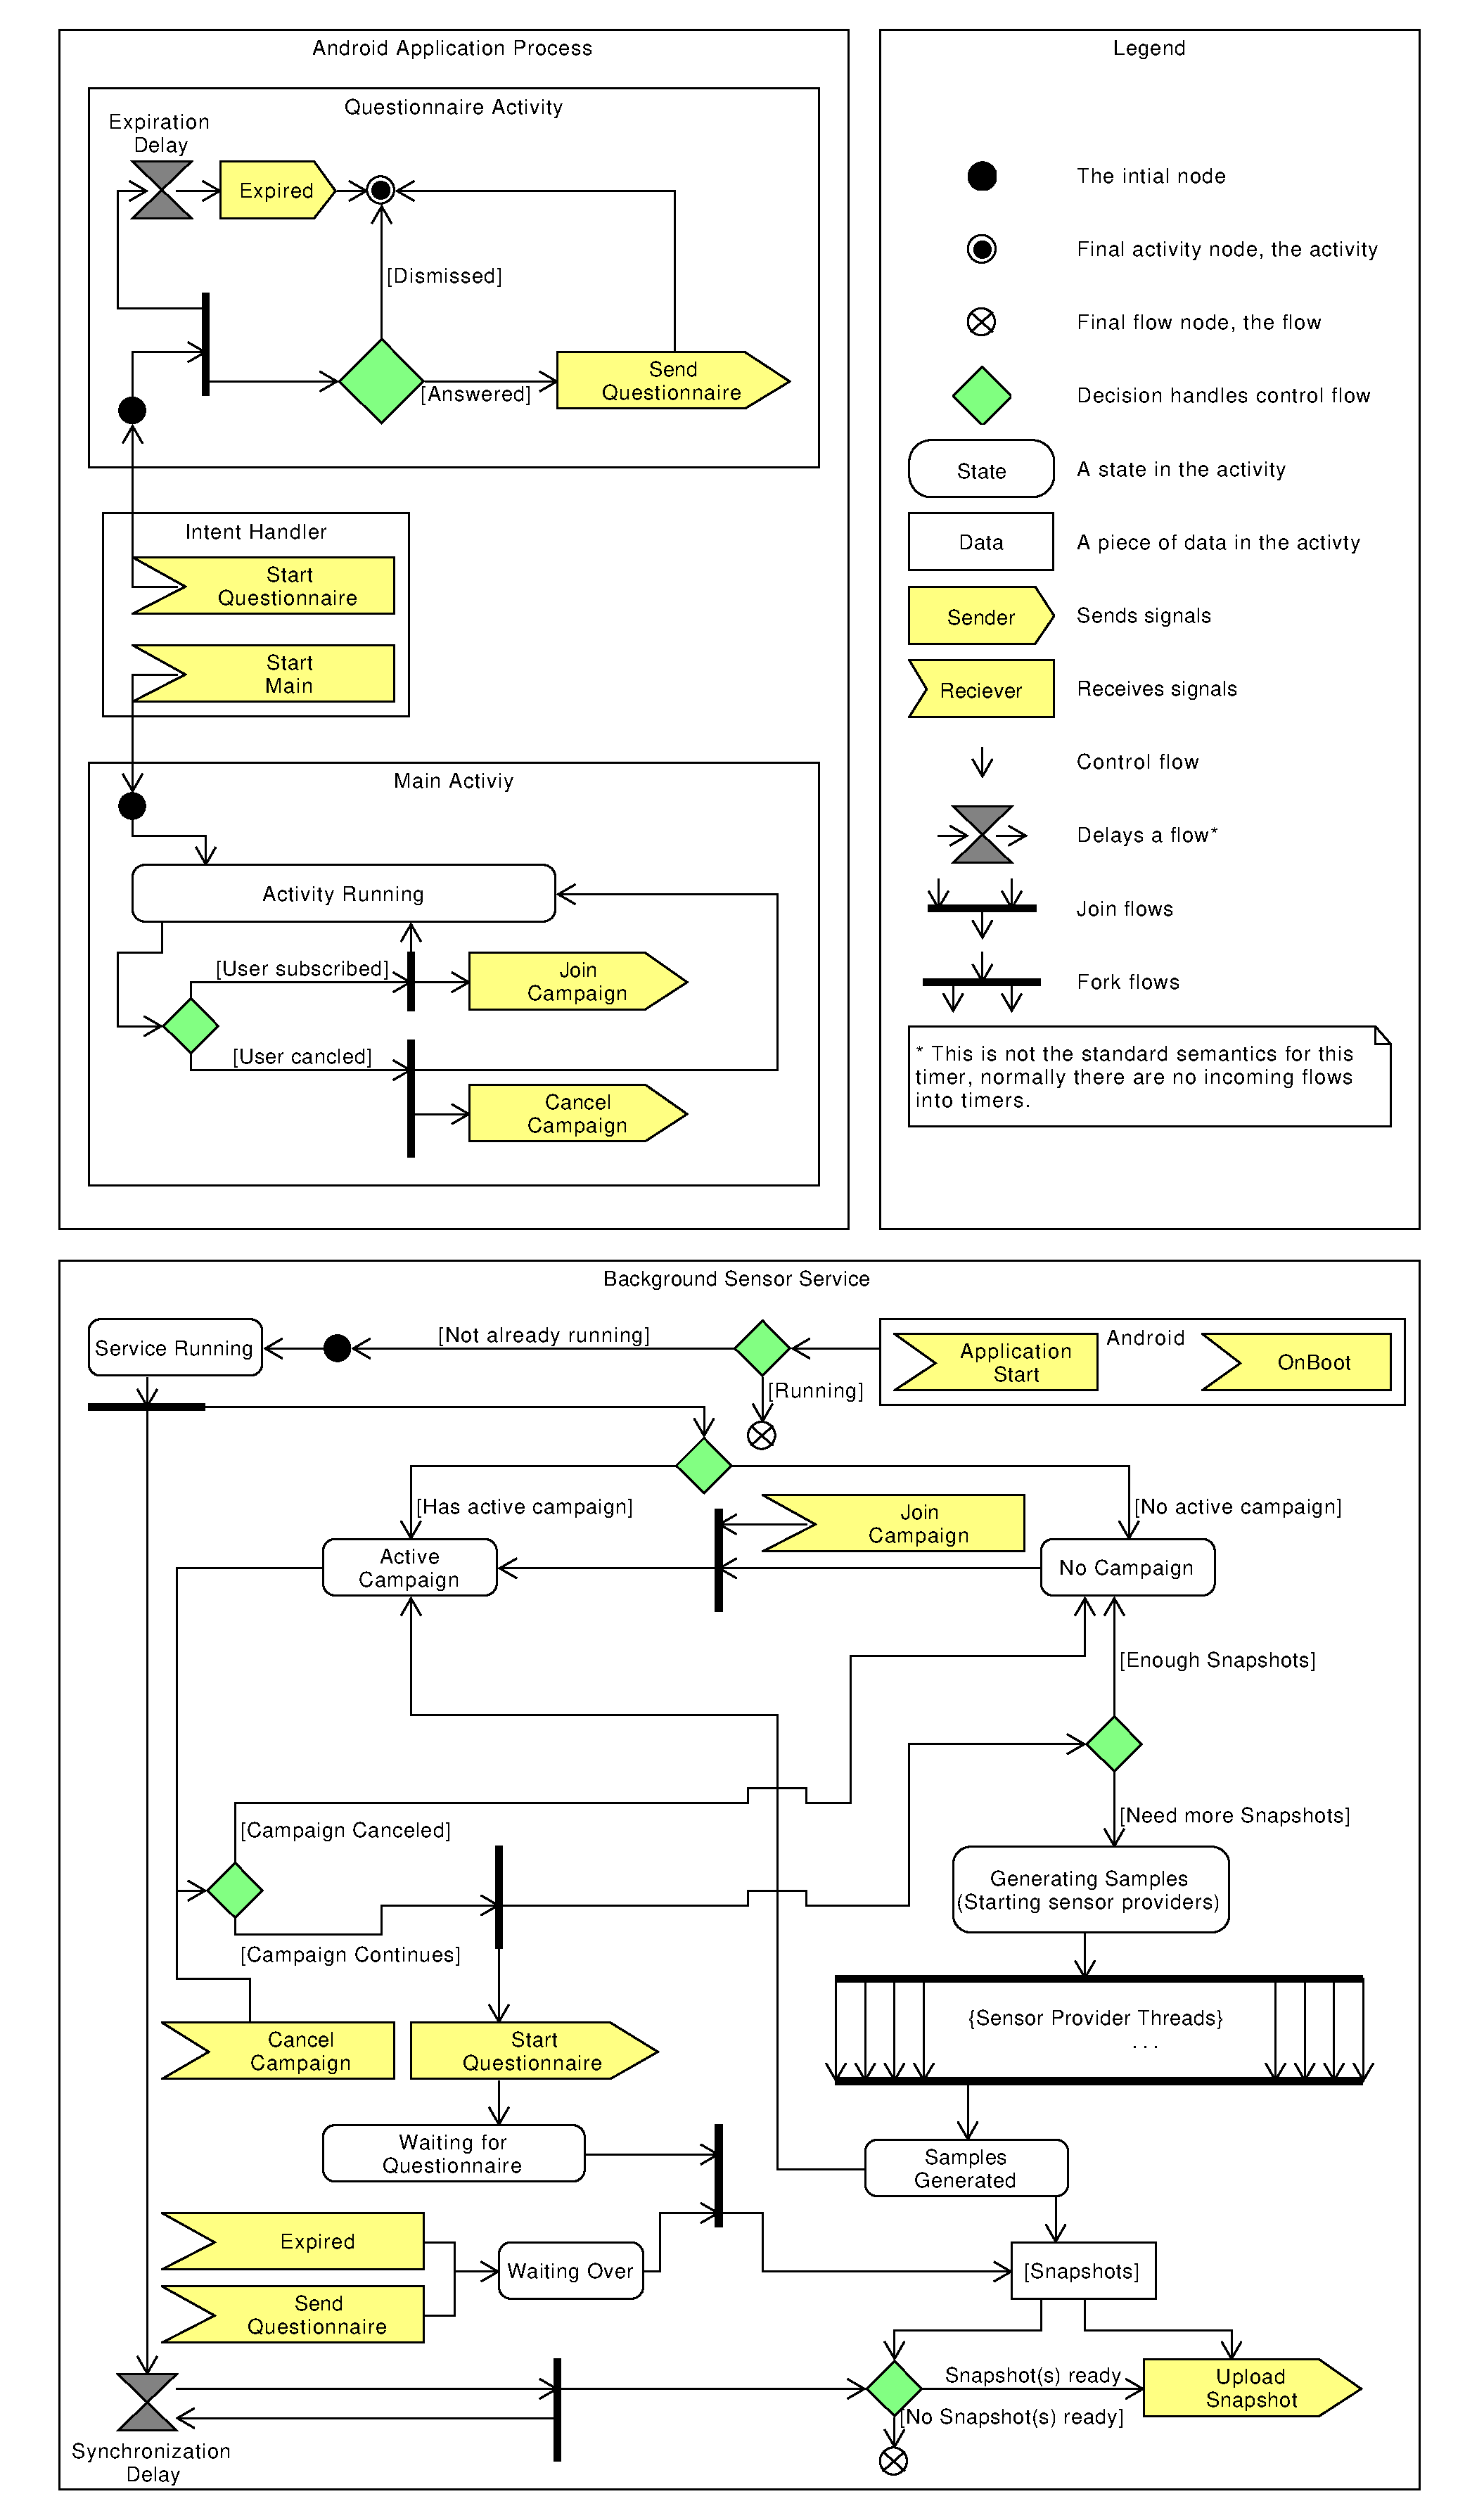
\includegraphics[width=0.9\textwidth]{graphic/backgroundsensorservice/lifecyclestuff}
    \caption{An overview of the mobile Application Components.}
    \label{fig:system_currency_and_lifecycle}
\end{figure}
\FloatBarrier